\chapter{Ottimizzazione delle performance}

Le performance delle applicazioni web sono un aspetto critico per garantire un'esperienza utente ottimale. Tempi di caricamento più veloci, maggiore reattività e una migliore gestione delle risorse sono fondamentali per mantenere gli utenti impegnati e soddisfatti. In questo contesto, l'ottimizzazione delle performance è diventata una priorità per gli sviluppatori web, che cercano di ridurre i tempi di caricamento, migliorare la fluidità delle applicazioni e ottimizzare l'uso delle risorse.

\paragraph{Panoramica}
Con l'evoluzione del web, abbiamo assistito a un enorme aumento del numero e delle dimensioni delle risorse inviate agli
utenti. Tra il 2011 e il 2019, il peso medio delle risorse è aumentato da 100 KB a 400 KB per i desktop e da 50 KB a
350KB per i dispositivi mobili. Mentre le dimensioni delle immagini sono aumentate da 250 KB a 900 KB per i desktop e
da 100 KB a 850 KB per i dispositivi mobili.


\section{Lazy Loading}

\subsection{Cos'è il Lazy Loading?}
Il Lazy Loading (conosciuto anche come caricamento asincrono) è una strategia per identificare le risorse come non bloccanti (non critiche) e caricarle solo quando necessario. È un modo per abbreviare la lunghezza del \href{https://developer.mozilla.org/en-US/docs/Web/Performance/Critical_rendering_path}{\textit{critical rendering path}}, che si traduce in tempi di caricamento della pagina ridotti.

\subsection{Panoramica}
As the web has evolved, we have come to see huge increases in the number and size of assets sent to users. Between 2011 and 2019, the median resource weight increased from ~100KB to ~400KB for desktop and ~50KB to ~350KB for mobile. While Image size has increased from ~250KB to ~900KB on desktop and ~100KB to ~850KB on mobile.

One of the methods we can use to tackle this problem is to shorten the Critical Rendering Path length by lazy loading resources that are not critical for the first render to happen. A practical example would be when you land on the home page of an e-commerce site with a link to a cart page/section, and none of the cart page's resources (such as JavaScript, CSS, and images) are downloaded until you navigate there.

\subsection{Strategie}
\href{https://developer.mozilla.org/en-US/docs/Web/Performance/Lazy_loading#strategies}{\textit{Strategies}}:

\subsection{Vantaggi e svantaggi del Lazy Loading}
\subsection{Impatto sulle performance}
\section{Code Splitting}
Il code splitting è una particolare implementazione del concetto di Lazy Loading che, in poche parole, consiste nel
dividere il codice JavaScript di grandi dimensioni in frammenti più piccoli chiamati \textbf{chunks}, in modo da
caricare solo ciò che è necessario per il funzionamento di una pagina durante l'avvio rimandando il caricamento degli
altri chunk fino a quando il codice non si rende necessario.  Questo approccio può migliorare notevolmente la reattività
del caricamento della pagina, in quanto riduce il tempo necessario per scaricare e interpretare il codice JavaScript.

\vspace{5mm}
\begin{figure}[H]
    \centering
    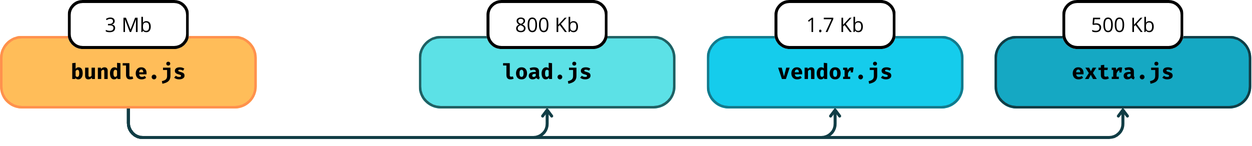
\includegraphics[width=0.8\textwidth]{performance/codesplitting.png}
    \caption{Code Splitting}
\end{figure}

\subsection{Vantaggi e svantaggi del Code Splitting}
Alcuni vantaggi del Code Splitting sono:
\begin{itemize}
    \item \textbf{Caricamento asincrono}: permette di caricare il codice JavaScript in modo asincrono, riducendo il payload iniziale.
    \item \textbf{Riduzione della dimensione del bundle}: riduce la dimensione del bundle JavaScript, migliorando le performance di caricamento.
    \item \textbf{Facilità di implementazione}: è possibile implementare il Code Splitting in modo semplice utilizzando strumenti come Webpack.
\end{itemize}

Di contro, il Code Splitting può comportare alcuni svantaggi:
\begin{itemize}
    \item \textbf{Overhead}: il caricamento asincrono dei chunk può comportare un overhead aggiuntivo.
    \item \textbf{Compatibilità}: alcune funzionalità del Code Splitting potrebbero non essere supportate da tutti i browser.
    \item \textbf{Debugging}: il debugging di applicazioni con Code Splitting può essere più complesso.
    \item \textbf{Cache}: il caching dei chunk può comportare problemi di cache invalidation.
    \item \textbf{Maggior numero di richieste HTTP}: il Code Splitting può comportare un maggior numero di richieste
    HTTP, soprattutto se la dimensione dei chunk è gestita in modo scorretto.
\end{itemize}


\section{Speculative loading}
\href{https://developer.mozilla.org/en-US/docs/Web/Performance/Speculative_loading}{Speculative Loading}

Lo speculative loading è una tecnica avanzata per migliorare le performance web attraverso lo svolgimento anticipato di azioni non ancora richieste dall'utente, come ad esempio fetch di dati da API, o il caricamento di pagine e risorse differenti da quelle attualmente visualizzate, prevedendo le azioni future dell'utente.

Questa tecnica è particolarmente utile per ridurre la percezione dei tempi di caricamento e migliorare l'esperienza utente, poiché anticipando il caricamento delle risorse che saranno necessarie in futuro, la percezione dell'utente sarà quella di un caricamento istantaneo, poiché le risorse saranno già disponibili in cache.

\subsection{Meccanismi di Speculative Loading}
Lo speculative loading può essere implementato in vari modi, a seconda delle esigenze dell'applicazione e delle risorse coinvolte. Alcuni esempi comuni includono:
\begin{itemize}
    \item \textbf{Prefetching}: Il prefetching è una tecnica che consiste nel caricare in anticipo le risorse necessarie per una determinata azione o pagina. Ad esempio, un browser potrebbe prefetchare le risorse di una pagina successiva, in modo che siano già disponibili in cache quando l'utente decide di visitarla. Questo riduce i tempi di caricamento e migliora l'esperienza utente.
    \item \textbf{Preloading}: Il preloading è simile al prefetching, ma si concentra sul caricamento di risorse critiche per la pagina attuale, come ad esempio immagini o script necessari per il rendering. Questo assicura che le risorse più importanti siano disponibili il prima possibile, migliorando la velocità di caricamento e la reattività dell'applicazione.
    \item \textbf{Prerendering}: Il prerendering è una tecnica che consiste nel caricare in background una pagina web completa, in modo che sia pronta per essere visualizzata istantaneamente quando l'utente decide di visitarla. Questo è particolarmente utile per le pagine di destinazione o le pagine più frequentemente visitate, in quanto riduce i tempi di caricamento e migliora l'esperienza utente.
    \item \textbf{Preconnecting}: Il preconnecting è una tecnica che consiste nel stabilire in anticipo una connessione con i server delle risorse, in modo da ridurre i tempi di latenza e migliorare le prestazioni. Ad esempio, un browser potrebbe preconnettersi ai server di un servizio di streaming video, in modo da ridurre i tempi di buffering durante la riproduzione.
    \item \textbf{Adaptive loading}: L'adaptive loading è una tecnica che si adatta dinamicamente alle condizioni di rete e alle risorse disponibili, caricando le risorse in base alla larghezza di banda e alla velocità di connessione dell'utente. Ad esempio, un'applicazione potrebbe caricare immagini di dimensioni diverse in base alla velocità di connessione, per garantire un'esperienza utente fluida anche su connessioni lente.
    \item \textbf{Service workers prefetching}: I service workers sono script JavaScript che girano in background nel browser e consentono di gestire in modo avanzato le richieste di rete e la cache delle risorse. I service workers possono essere utilizzati per implementare tecniche di speculative loading, come il prefetching delle risorse o il caching delle risposte, per migliorare le performance e l'esperienza utente.
\end{itemize}

\subsection{Selezione delle risorse da precaricare}
La selezione delle risorse da precaricare viene principalmente svolta in due modalità.
Innanzitutto, alcuni browser prerenderizzano automaticamente le pagine in base a determinate euristiche per migliorare le performance. Ad esempio, Chrome può prerenderizzare pagine quando vengono digitate stringhe nell'indirizzo, se ha una forte previsione che l'utente le visiterà. Inoltre, può prerenderizzare pagine di risultati di ricerca quando il motore di ricerca lo richiede, utilizzando la \href{https://developer.mozilla.org/en-US/docs/Web/API/Speculation_Rules_API}{Speculation Rules API}

Successivamente, gli sviluppatori possono fornire indicazioni specifiche attraverso varie funzionalità della piattaforma, decidendo autonomamente e in base ai propri criteri le strategie, tra quelle illustrate in precedenza, da adottare. Ad esempio, è possibile utilizzare il tag \texttt{<link rel="prefetch">} per indicare al browser di precaricare una risorsa, o il tag \texttt{<link rel="prerender">} per indicare di prerenderizzare una pagina.



\section{Impatto sulle performance}

Vantaggi di Code Splitting e Lazy Loading:
\begin{itemize}
    \item Riduzione dei tempi di caricamento iniziale: Code splitting divide il codice JavaScript in moduli che vengono caricati solo quando necessari, permettendo alle pagine di caricarsi più velocemente. Lazy loading, invece, posticipa il caricamento di risorse (come immagini o video) fino a quando non sono effettivamente visualizzati, riducendo la quantità di dati inizialmente scaricati
    \item Migliore esperienza utente: I tempi di caricamento più rapidi e la maggiore reattività dell'applicazione consentono agli utenti di iniziare a interagire con il sito prima che tutte le risorse siano caricate. Questo è particolarmente utile per siti con molti contenuti multimediali o applicazioni JavaScript complesse
    \item Riduzione dell'uso di banda: Lazy loading carica solo le risorse necessarie, ottimizzando il consumo di banda, specialmente su dispositivi mobili e connessioni lente
    \item Migliore gestione delle risorse: Queste tecniche riducono il carico sui server e migliorano la gestione delle risorse di memoria, poiché vengono gestite in modo più efficiente le richieste di risorse non immediatamente necessarie
\end{itemize}

Sfide e svantaggi:
\begin{itemize}
    \item LCP peggiorato: Lazy loading può peggiorare il Largest Contentful Paint (LCP) su alcune pagine, poiché ritarda il caricamento delle immagini necessarie nella parte visibile (above-the-fold). Studi su WordPress hanno mostrato che disabilitare il lazy loading per le immagini sopra la piega può migliorare significativamente il LCP
    \item Gestione complessa: Implementare correttamente code splitting e lazy loading richiede una comprensione approfondita di quando e come dividere il codice o posticipare il caricamento delle risorse. Configurazioni errate possono portare a problemi di performance o alla mancata visualizzazione di contenuti essenziali
    \item Possibili conflitti con altre ottimizzazioni: Code splitting e lazy loading devono essere ben bilanciati con altre tecniche come il prefetching e il caching, per evitare conflitti di banda che potrebbero rallentare l'esperienza utente
\end{itemize}

\paragraph{Studi sull'impatto delle performance}
Alcuni studi dimostrano l'importanza di implementare correttamente queste tecniche. Ad esempio, un test su WordPress ha rilevato che disabilitare il lazy loading migliorava il LCP su pagine di archivio del 13-15\%, mentre l'abilitazione del lazy loading riduceva la quantità di dati immagine caricati, migliorando la banda utilizzata, ma a scapito di un ritardo nel caricamento delle immagini principali

Nel complesso, quando usate correttamente, queste tecniche forniscono un ottimo equilibrio tra prestazioni e esperienza utente, ma richiedono un'implementazione oculata per evitare effetti indesiderati.


